\chapter{Cadre du projet}
\section*{Introduction}
\addcontentsline{toc}{section}{Introduction }
Dans ce premier chapitre, nous plongeons dans le contexte global de notre projet au sein d'Avaxia Group. Cette section établit les bases en présentant le cadre général du projet, en soulignant les objectifs que nous nous efforçons d'atteindre.

% Une section

% Exemple d'une section qui porte une référence à une bibliographie
% NB: il faut bien suivre le syntaxe pour ne pas tomber dans le cas où il y a une référence dans la table des matières.
\section {Context général du projet}
\par Ce projet s'inscrit dans le cadre du stage de fin d'études d'ingénieur au sein de la société Avaxia Group, se déroulant de Février 2024 à Mai 2024, dans l'objectif de l'obtension de diplôme national d'ingénieur de l'Institut Supérieur d'Informatique (ISI). 
"Notre mission centrale consiste à contribuer à la réalisation du projet intitulé "", en apportant notre expertise et notre contribution essentielle
\section[Organisme d'accueil]{Organisme d'accueil}
\subsection{Présentation générale de Avaxia Group}
% NB: il faut annoncer la figure dabord.
% Pour faire appel à une figure, il suffit d'utiliser le label comme suit :
\par Avaxia Group, une entreprise de conseil en technologie créée en 1998 et ayant son siège à Dubaï, étend actuellement sa présence mondiale avec des bureaux au Japon et en Tunisie, et de futurs emplacements prévus au Canada, en France et à Dakar. Avaxia Group se spécialise dans les solutions middleware, la gestion des infrastructures système, ainsi que dans le conseil fonctionnel, couvrant des domaines tels que l'architecture, l'intégration et les opérations \cite{avaxia}.
\subsection{Les services de Avaxia Group \cite{serAvaxia}}
\par Avaxia Group opère sur le vaste marché international, avec une présence dans de nombreux pays. L'entreprise propose une gamme diversifiée de services, notamment les suivants :

\setlist[itemize]{label=$\bullet$}
\begin{itemize}
\setlist[itemize]{label= \textbf{-}}

    \item \textbf{Expertise Technique en SAP: }
    \begin{itemize}
        \item  Gestion de l'infrastructure.
        \item  Optimisation et amélioration des performances.
        \item  Conception et architecture du paysage SAP.
        \item  Installation des systèmes, configuration et mises à niveau.
        \item  Assistance technique 24/7.
    \end{itemize}
    % 
    \item \textbf{Conseil Fonctionnel : }
            \begin{itemize}
                \item  Gestion fonctionnelle du déploiement et planification des tests.
                \item  Conception de solutions métier pour le déploiement de nouveaux modules SAP.
        
            \end{itemize}
     \item \textbf{ Solutions Logicielles Personnalisées :}
            \begin{itemize}
                \item  Conception et développement de solutions logicielles utilisant des technologies telles que Java J2E, DELL BOOMI Flow, Salesforce et SAP Fiori.
            \end{itemize}
         \item \textbf{Intégration des Systèmes :}
            \begin{itemize}
                \item  Intégration de données et gestion des flux de données.
                \item Intégration d'applications métier.
                \item Développement et gestion d'API : DELL BOOMI, Atmosphère.
            \end{itemize}
    \item \textbf{Ingénierie des Données :}
            \begin{itemize}
                \item  Modélisation, découverte, traitement, visualisation et exploration des données, ainsi que gestion du Big Data.
            \end{itemize}
    \item \textbf{Nouvelles Technologies :}
            \par Création et déploiement de solutions logicielles d'entreprise en utilisant les dernières technologies, notamment :
            \begin{itemize}
                \item  Apprentissage automatique (Machine Learning).
                \item Réalité virtuelle (VR).
                \item Réalité augmentée (AR).
                \item Internet des objets (IoT).
            \end{itemize}
    
\end{itemize}
\par Cette gamme diversifiée de services reflète l'engagement d'Avaxia Group à fournir des solutions techniques avancées et à rester à la pointe de l'innovation pour répondre aux besoins variés de ses clients à l'échelle mondiale.


\section{\'Etude du projet}
\par Dans cette section nous explorons en détail  l'etude de ce projet toutes en commmançant par les raisons fondamentales ayant motivé le développement de notre solution et les spécifications de cette derniére ainsi que son objectif.
\subsection{Problématique}
\par Avec l'avènement des technologies de cloud computing et des entrepôts de données modernes tels que Snowflake, les entreprises disposent désormais d'une flexibilité et d'une évolutivité inégalées pour la gestion et l'analyse de leurs données. 
Cependant, cette transition vers le cloud présente des défis spécifiques en termes de performance, de coûts, et de surveillance des opérations. 
\par Dans ce contexte, Avaxia Group se trouve confrontée à des problématiques particulières liées à l'utilisation de Snowflake, son principal entrepôt de données telque : 
\begin{itemize}
    \item \textbf{Gestion des performances: } \par - Avaxia Group constate des délais dans l'exécution des requêtes et des temps de traitement prolongés lors de l'utilisation de Snowflake. Ces problèmes impactent directement la productivité des équipes et la satisfaction des utilisateurs finaux.
    \par - Les requêtes SQL complexes ou mal optimisées peuvent engendrer des goulets d'étranglement et des inefficacités dans l'utilisation des ressources de Snowflake, nécessitant une surveillance et une optimisation constantes.
    \item \textbf{Maîtrise des coûts:} \par - Les coûts associés à l'utilisation de Snowflake peuvent rapidement augmenter en raison d'une gestion inadéquate des ressources. Avaxia Group doit donc trouver des moyens de maîtriser ces coûts tout en garantissant des performances optimales pour ses opérations.
    \item \textbf{Surveillance et analyse des opération:} \par - Pour assurer le bon fonctionnement de ses opérations Snowflake, Avaxia Group a besoin d'une solution de surveillance avancée pour détecter les anomalies, identifier les goulets d'étranglement et optimiser les performances.
    \par De plus, une analyse approfondie des métriques opérationnelles telles que le temps d'exécution des requêtes, l'utilisation des ressources et les performances des entrepôts est essentielle pour optimiser l'efficacité et l'efficience des opérations.
\end{itemize}

\subsection{Analyse et critique de l'existant}
Dans cette section, nous passerons en revue les fonctionnalités, les avantages et les limitations de chaque solution, en mettant en lumière les lacunes qui ont conduit au développement de notre propre solution de monitoring des opérations Snowflake chez Avaxia Group.
\subsubsection{Analyse de l'existant}
\par L'analyse de l'existant est une étape cruciale dans le processus de développement de notre solution de monitoring des opérations sur Snowflake.
C'est pour céla, nous allons entammer l'analyse les outils existants utilisés pour surveiller et analyser les opérations sur les divers plateformes de l'analyse des données et le data warehousing cloud
\begin{itemize}
    \item\textbf{Snowflake account usage dashboard :}  est un outil intégré qui fournit des informations sur l'utilisation de Snowflake, telles que le nombre de sessions utilisateur, 
    la quantité de données stockées et le temps CPU utilisé.
    Il offre une vue rétrospective des opérations passées, permettant aux utilisateurs de comprendre l'utilisation historique de la plateforme. 
    \par La figure \textbf{\ref{fig:SAU}} suivante illustre une partie de cette dashboard:
        %code image
            \begin{figure}[H]
            \centering
            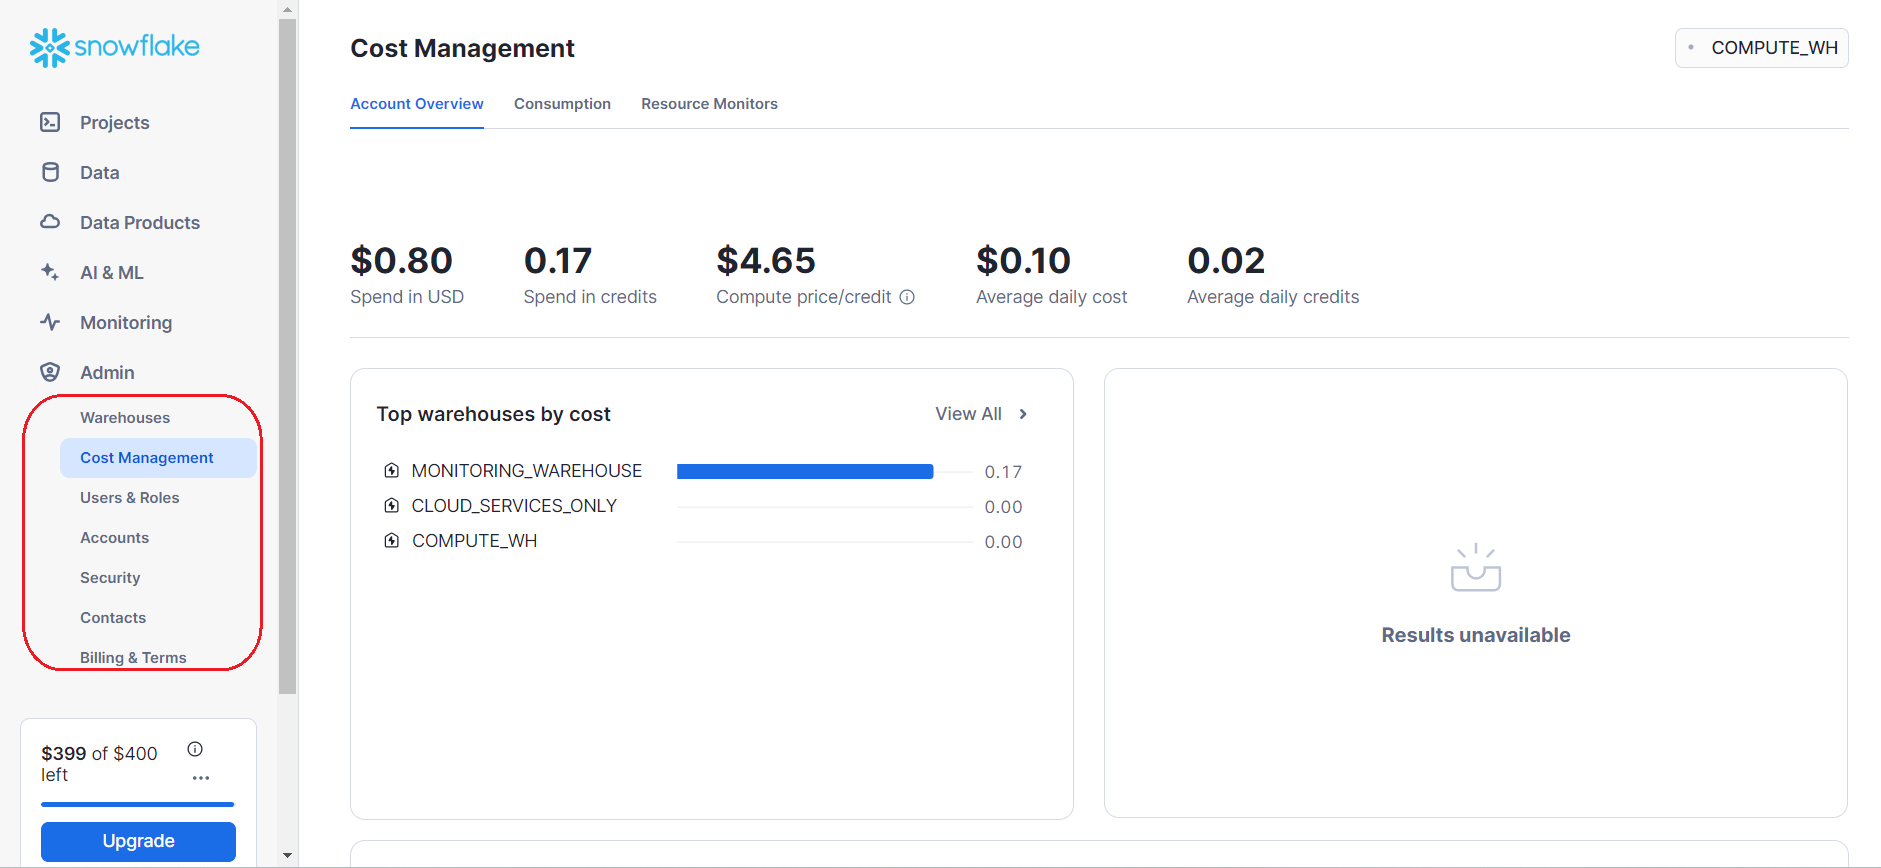
\includegraphics[width =13cm, height=7.5cm]{img/captures/account_usage}
            \caption{Snowflake account usage dashboard}
            \label{fig:SAU}
            \end{figure}
        %fin
    \item\textbf{Snowflake Information Schema:} est une collection de vues système qui fournissent des métadonnées sur les objets et les opérations effectuées dans un compte Snowflake. 
    Ces vues offrent une granularité élevée pour examiner les détails des requêtes SQL exécutées, les performances des entrepôts de données et d'autres aspects des opérations Snowflake. 
    \par La figure \textbf{\ref{fig:info}} suivante illustre une partie de cette dashboard:
        %code image
            \begin{figure}[H]
            \centering
            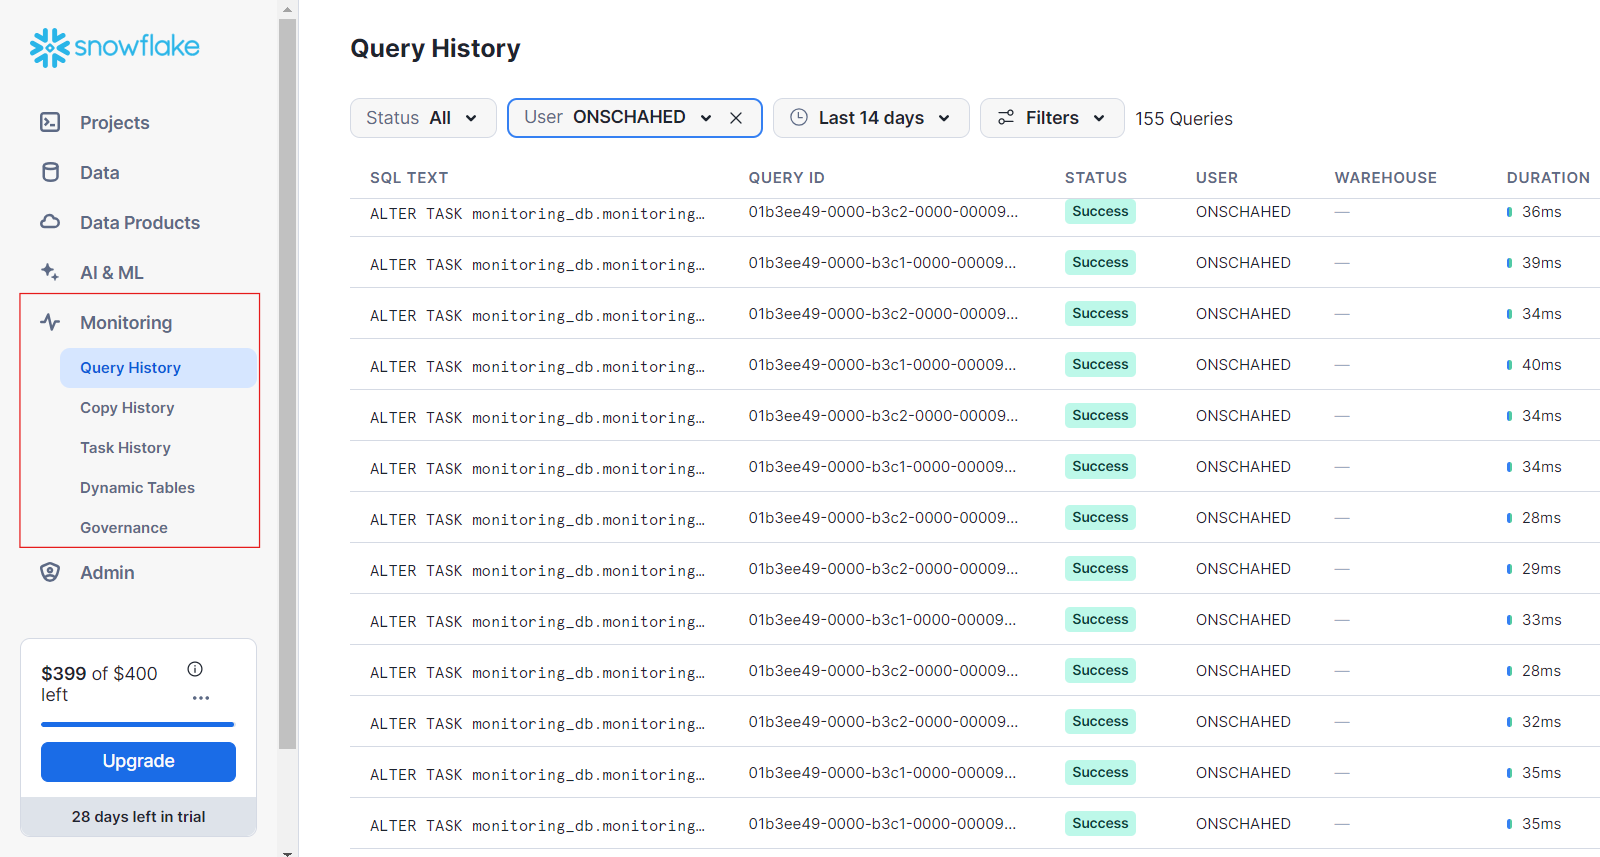
\includegraphics[width =13cm, height=7.5cm]{img/captures/info}
            \caption{Snowflake account usage dashboard}
            \label{fig:info}
            \end{figure}
        %fin
    \item\textbf{Google BigQuery:} est une autre option populaire pour le stockage et l'analyse des données dans le cloud. 
    Il offre des fonctionnalités avancées telles que le traitement massivement parallèle et la capacité à exécuter des requêtes SQL complexes sur de grands ensembles de données. 
    \par La figure \textbf{\ref{fig:BQ}} suivante illustre une partie de tableau de bord de BigQuery :
        %code image
            \begin{figure}[H]
            \centering
            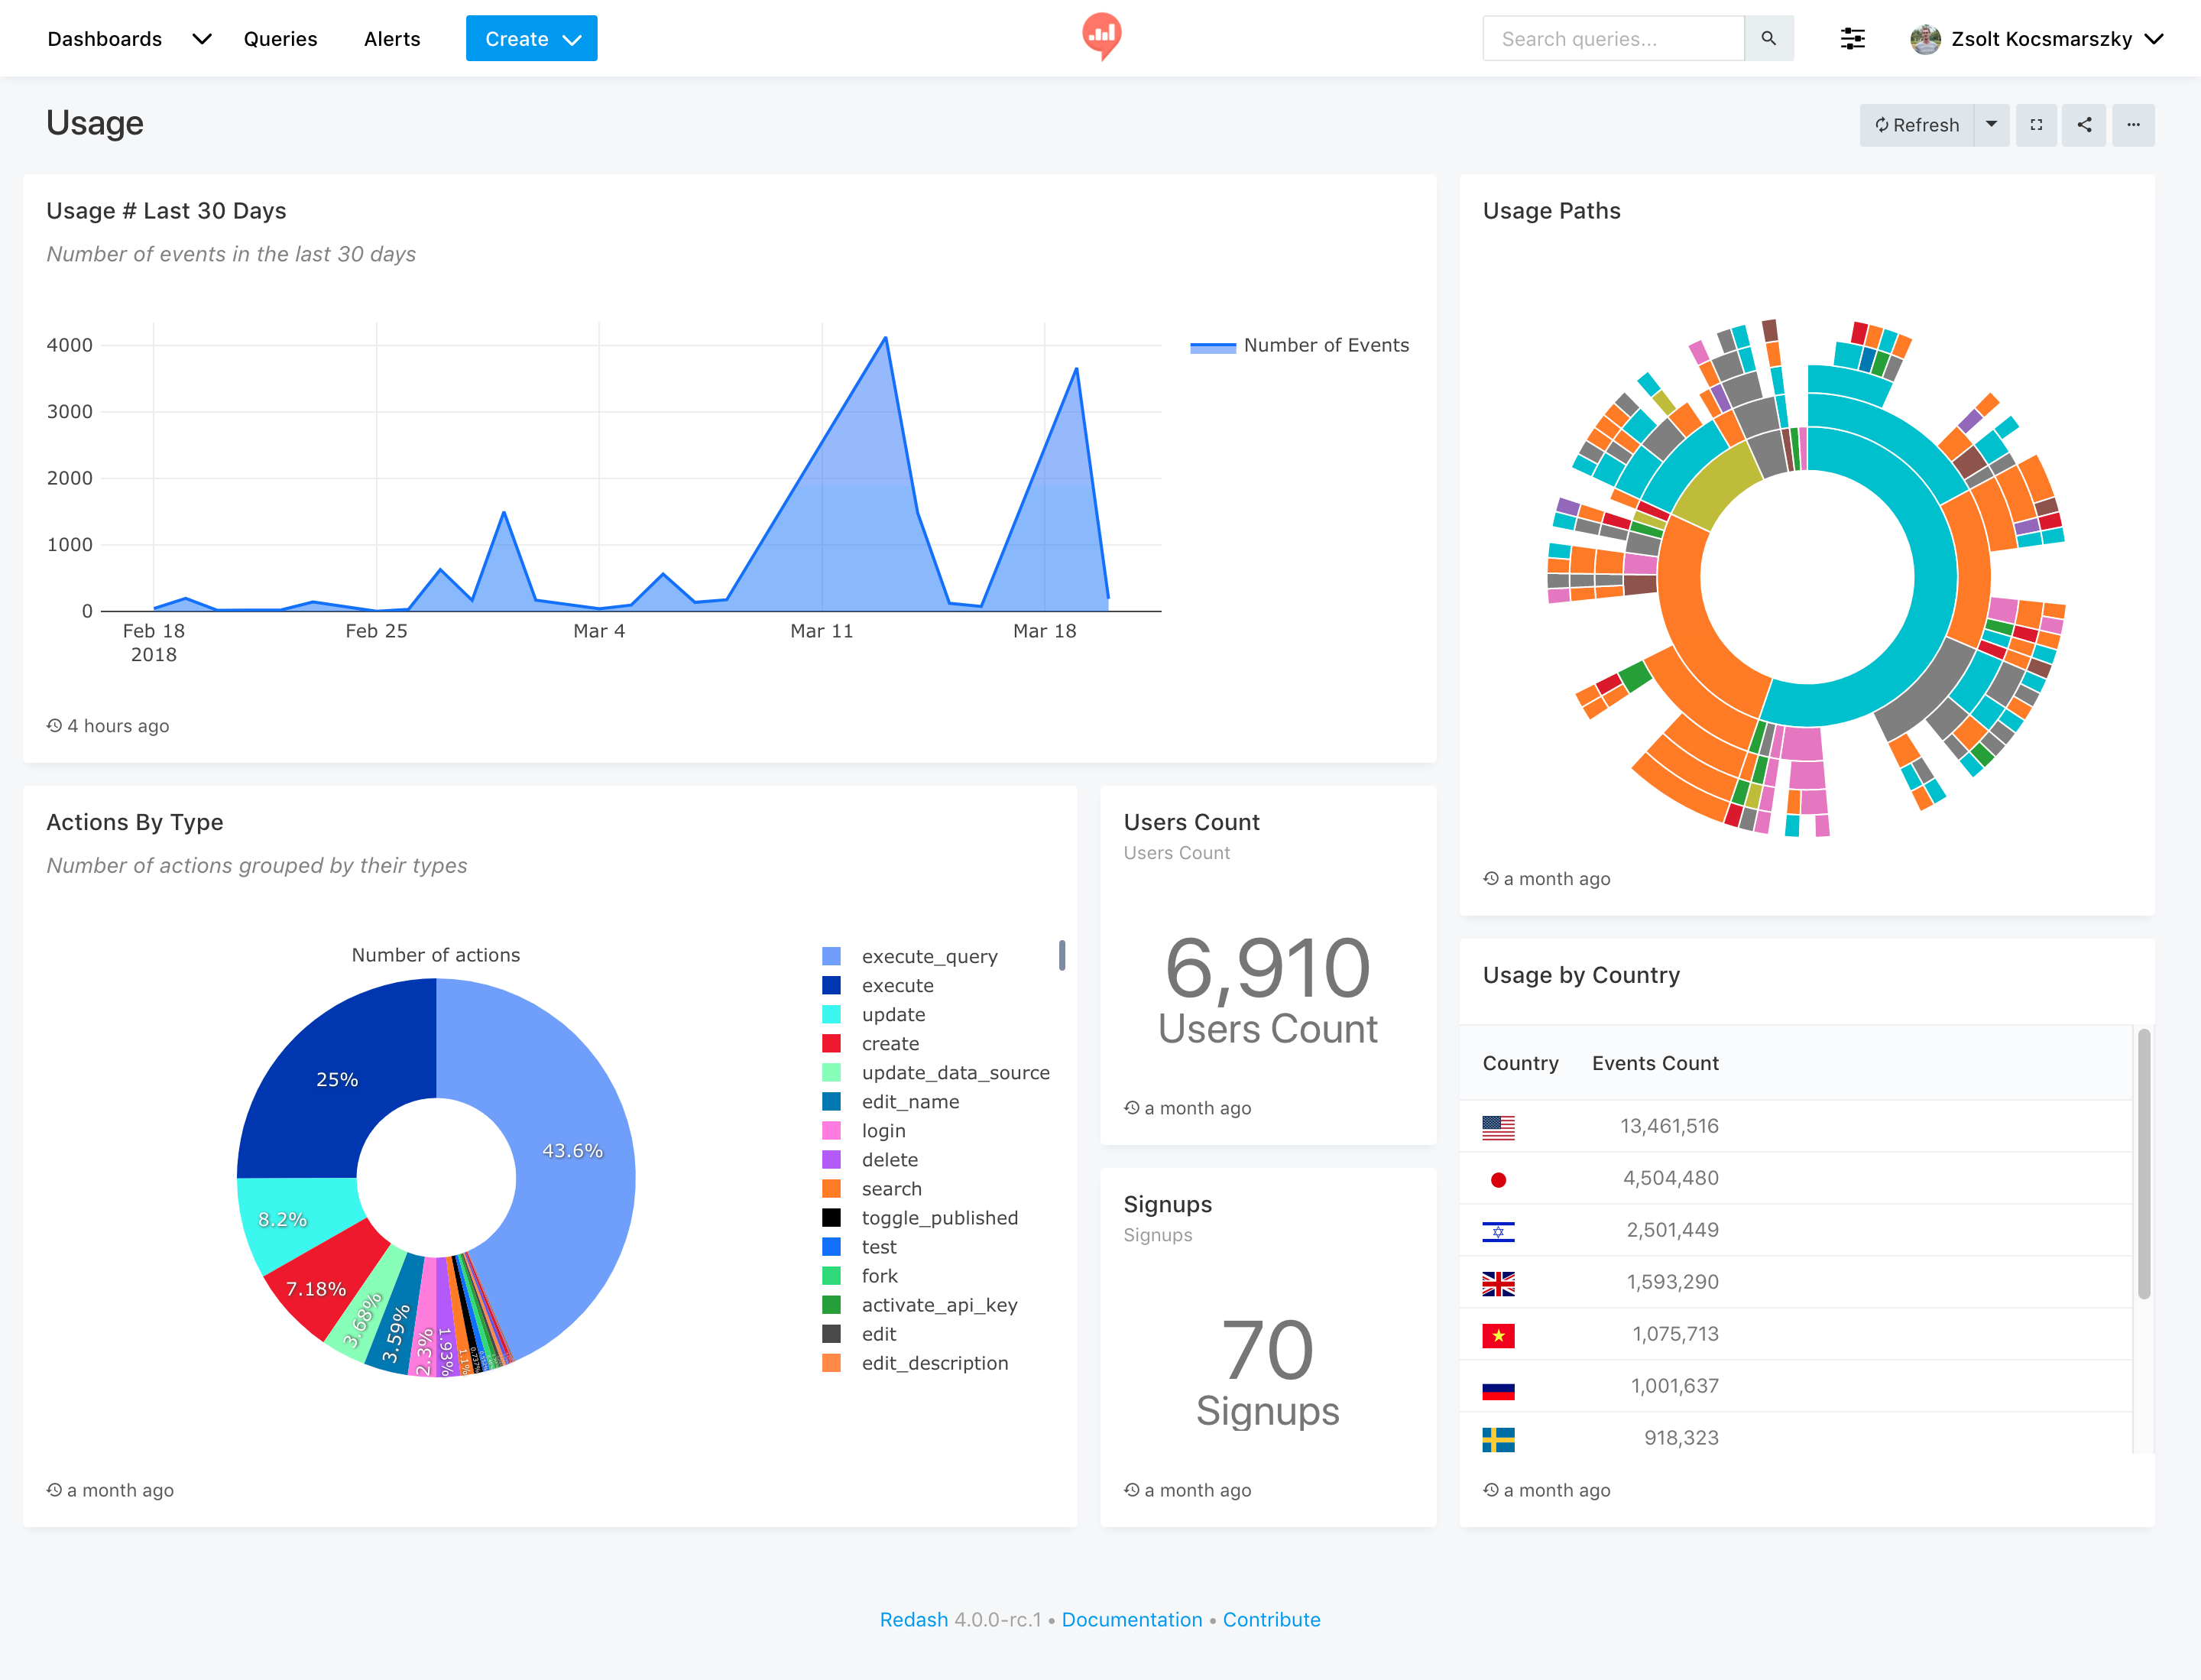
\includegraphics[width =13cm, height=7.5cm]{img/captures/bigquery}
            \caption{Tableau de bord de "Google BigQuery"}
            \label{fig:BQ}
            \end{figure}
        %fin

    \item\textbf{Amazon Redshift:} est un entrepôt de données cloud basé sur PostgreSQL, conçu pour gérer de gros volumes de données et exécuter des analyses complexes.
    Il offre des performances élevées et une extensibilité, mais son modèle de tarification basé sur l'utilisation des ressources peut entraîner des coûts supplémentaires pour les entreprises
    \par La figure \textbf{\ref{fig:RS}} suivante illustre le tableau de bord de ResShift:
        %code image
            \begin{figure}[H]
            \centering
            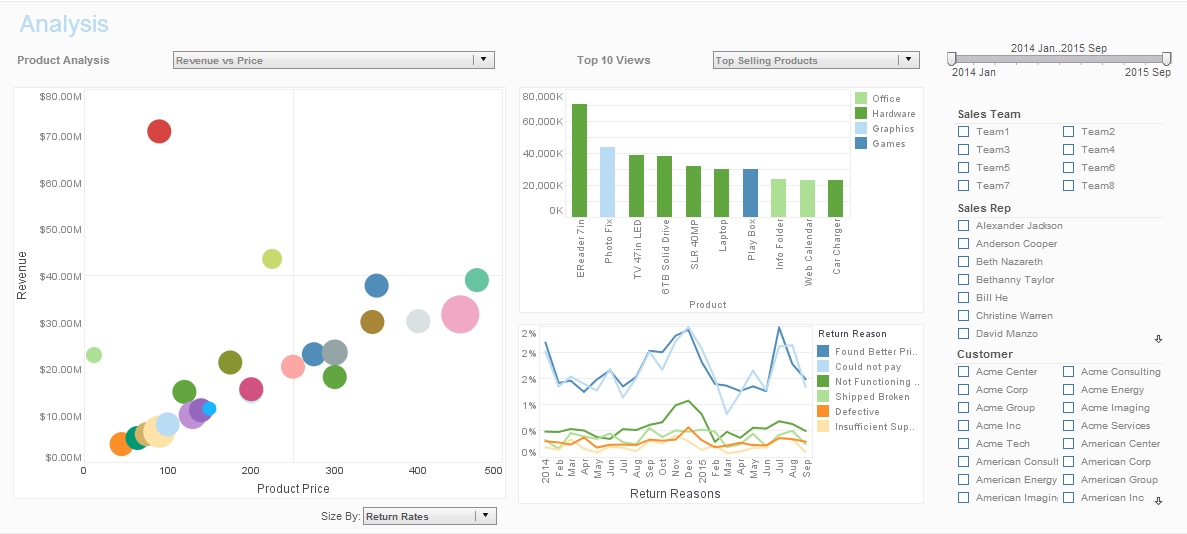
\includegraphics[width =13cm, height=7.5cm]{img/captures/redshift}
            \caption{Tableau de bord de "Amazon Redshift"}
            \label{fig:RS}
            \end{figure}
        %fin
\end{itemize}
\subsubsection{Critique de l'existant}
\par Dans cette section, nous allons examiner de manière critique les outils actuellement utilisés dans le domaine de l'analyse de données, afin de fournir une base solide pour concevoir une solution qui surmonte les limitations et offre une valeur ajoutée significative à Avaxia Group et à ses clients.
\begin{itemize}
    \item\textbf{Manque d'analyse prédictive: }l'un des principaux défauts des outils actuellement disponibles est leur incapacité à fournir une analyse prédictive des performances de Snowflake. 
    Les tableaux de bord existants, tels que le Snowflake Account Usage Dashboard, offrent une vue rétrospective des opérations passées, mais ne fournissent pas d'informations sur les tendances futures ou les possibles goulots d'étranglement.

    \item\textbf{Complexité des outils: }les outils de surveillance existants, comme le Snowflake Information Schema, sont souvent complexes à utiliser et nécessitent des compétences techniques avancées pour interpréter les données fournies. 
    Cette complexité peut rendre difficile la compréhension des métriques et la prise de décisions éclairées par les équipes opérationnelles.
    ( par exemple dans un workflow si une certaine tache est échouée, les indicateurs disponibles sur snowflake ne peuvent pas identifier ou exactement le workflow est suspendu de façon à rendre les choses plus compliqué pour les utilisaturs de Snowflake de détecter les anomalies.)

    \item\textbf{Personnalisation limitée: }les options de personnalisation offertes par les outils existants sont souvent limitées. 
    Par exemple, Google BigQuery propose des fonctionnalités avancées, mais la personnalisation des tableaux de bord et des rapports est restreinte. Cela peut être un obstacle pour les entreprises ayant des besoins spécifiques en matière de surveillance et d'analyse des performances.

    \item\textbf{Coûts supplémentaires: } enfin, certains outils, comme Amazon Redshift, peuvent entraîner des coûts supplémentaires importants pour les entreprises. La tarification basée sur l'utilisation des ressources peut rapidement augmenter, surtout si les entreprises ne surveillent pas activement leur utilisation. Cela peut constituer une barrière financière pour les petites et moyennes entreprises souhaitant utiliser ces outils de surveillance.


\end{itemize}
\subsection{Solution proposée}
\par Notre solution pour résoudre les défis auxquels Avaxia Group est confronté dans l'utilisation de Snowflake repose sur la conception et l'implémentation d'un système de surveillance et d'optimisation des opérations exhaustif. Cette solution se décompose en plusieurs composants clés, chacun ciblant des aspects spécifiques des problématiques identifiées :
\begin{itemize}
    \item Développement d'algorithmes d'optimisation des requêtes SQL afin de de réduire les temps d'exécution et de minimiser les goulets d'étranglement dans l'utilisation des ressources de Snowflake.
    \item Mise en place de stratégies de monitoring en temps réel cela permettra d'identifier rapidement les problèmes de performance et de prendre des mesures correctives efficaces.
    \item Développement d'outils d'analyse avancée des coûts Cette analyse approfondie aidera nos utilisateurs finaux à mieux comprendre ses dépenses et à trouver des opportunités d'optimisation pour réduire les coûts tout en maintenant des performances élevées.
    \item la mise en place de politiques de gestion des ressources pour optimiser l'utilisation des ressources de Snowflake. Des stratégies telles que le dimensionnement automatique des entrepôts de données et l'optimisation de l'utilisation des crédits de calcul seront explorées.
    \item Développement des tableaux de bord interactifs et riches en informations pour permettre à Avaxia Group et à ses clients de surveiller en temps réel les performances de leurs opérations Snowflake. Ces tableaux de bord fourniront des indicateurs clés de performance, des graphiques et des visualisations pour faciliter la détection des anomalies et la prise de décisions éclairées.
    \item Utilisation de techniques d'analyse avancée des données opérationnelles pour permettre aux utilisateurs  d'identifier les opportunités d'amélioration et d'optimisation de leurs opérations, renforçant ainsi leur compétitivité et leur efficacité.
\end{itemize}


\section{Choix méthodologique}

\par Le choix de la méthode Kanban pour la gestion de notre projet est le fruit d'une réflexion stratégique minutieuse, loin d'être aléatoire. Kanban, qui tire son origine du terme japonais signifiant "tableau", se démarque par sa flexibilité, sa transparence et sa focalisation sur l'amélioration constante.

\par Dans le cadre de notre projet, Kanban s'impose naturellement comme le choix optimal. 
Cette méthode permet une gestion visuelle et en temps réel des tâches et des flux de travail, une caractéristique cruciale pour un projet centré sur l'analyse de données et la visualisation.
 Chaque étape de notre processus, de la collecte des données à la présentation des résultats, trouve une représentation claire et concise dans le tableau Kanban.

\par De surcroît, Kanban promeut une approche itérative et progressive, parfaitement en harmonie avec notre objectif d'amélioration continue. 
Elle autorise une gestion fluide et adaptable des tâches, offrant la souplesse nécessaire pour ajuster notre plan en fonction des découvertes et des besoins changeants du projet.

\par En optant pour Kanban, nous mettons l'accent sur la transparence et la communication au sein de l'équipe. 
Chacun dispose d'une vision limpide de l'état d'avancement du projet, favorisant ainsi la collaboration et l'engagement de tous les membres.

\par En résumé, la méthode Kanban s'impose comme un choix stratégique judicieux pour notre projet, offrant un cadre solide pour une gestion efficace, transparente et itérative, tout en servant l'objectif fondamental d'amélioration continue de la performance de l'équipe Avaxia.

\section*{Conclusion}
\addcontentsline{toc}{section}{Conclusion}
   À la clôture de ce chapitre initial,
    nous avons jeté les fondements pour la compréhension complète de la sphère du projet. Cette phase est cruciale pour cadrer les enjeux et les perspectives qui guident notre travail. Dans le prochain chapitre, nous explorerons en détail l'analyse et la spécification des besoins, une étape essentielle pour la réalisation de notre projet.